\section{Optique géo. surfaces courbes}
\vspace{-2\baselineskip}
\subsection{Dioptre}
\begin{tabular}{ll}
    Lentille &  \(\frac{n_i}{s_o}+\frac{n_t}{s_i}=\frac{n_t-n_i}{R}\)\\[8pt]
    Miroir & \(\frac{1}{s_o}+\frac{1}{s_i}=\frac{2}{R}=\frac{1}{f}\)
\end{tabular}

% \[\frac{n_i}{s_o}+\frac{n_t}{s_i}=\frac{n_t-n_i}{R}\]
% \subsubsection{Cas particulier: Miroir}
% \[\frac{1}{s_o}+\frac{1}{s_i}=\frac{2}{R}\]

% \subsubsection{Distance focale}
% \[\frac{1}{s_o}+\frac{1}{s_i}=\frac{2}{R}=\frac{1}{f}\]
\subsection{Foyers}
\begin{tabular}{ll}
    Objet & \(f_o = \frac{n_i R}{n_t-n_i} \) \\
    Image & \(f_i = \frac{n_t R}{n_t-n_i} \)
\end{tabular}

\subsection{Lentille mince}
\begin{align*}
    \frac{1}{s_i}+\frac{1}{s_o}&=\frac{n_l-n_a}{n_a}\qty(\frac{1}{R_1}+\frac{1}{R_2})\\
    \frac{1}{s_i}+\frac{1}{s_o}&=(n_{la}-1)\qty(\frac{1}{R_1}+\frac{1}{R_2})
\end{align*}

\subsection{Lentille épaisse}
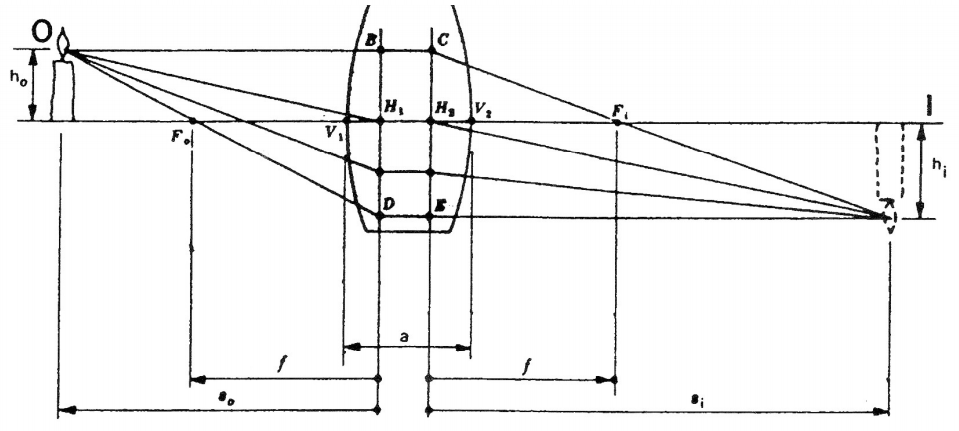
\includegraphics[width=.45\textwidth]{fig/thk_lens.PNG}
\[\frac{1}{s_i}+\frac{1}{s_o}=\frac{1}{f} = (n_{la}-1)\qty(\frac{1}{R_1}-\frac{1}{R_2}+\frac{(n_{la}-1)a}{n_{la}R_1R_2})\]
% $a$ est l'épaisseur de la lentille.
\subsubsection{Plans principaux}
$V$ vers $H$ dans le sens de la propagation.
\begin{align*}
    \overline{V_1H_1} &= \frac{-f(n_{la}-1)a}{R_2n_{la}}\\
    \overline{V_2H_2} &= \overline{V_1H_1}\frac{R_2}{R_1}
\end{align*}

\subsection{Grandissement}
\begin{tabular}{ll}
    Grandissement &  \(g_t = \frac{-n_i s_i}{n_t s_o} = \frac{h_i}{h_o}=\frac{-s_i}{s_o}\) \\[8pt]
    Grandissement total & \(g_t=g_{t_{1}}\times g_{t_{2}} \times \ldots = \frac{h_i}{h_o}\)
\end{tabular}

\subsection{Combinaison de lentilles}
\centering
\includegraphics[trim={.75cm 0 1cm 0},clip=true, width=.4\textwidth]{fig/lens_comb.tex}
\[s_{o_2}=d_a-s_{i_1}\]

\raggedright